\section{Introduction}

%\subsection{Variable assignment}

%\subsection{Variable assignment}

\begin{frame}[fragile]
\frametitle{Variable assignment}

    Python is a dynamical binding and typing language, contrary to C/C++, Java and Fortran (source: \href{https://pythonconquerstheuniverse.wordpress.com/2009/10/03/static-vs-dynamic-typing-of-programming-languages/}{pythonconquerstheuniverse})

    \begin{center}
    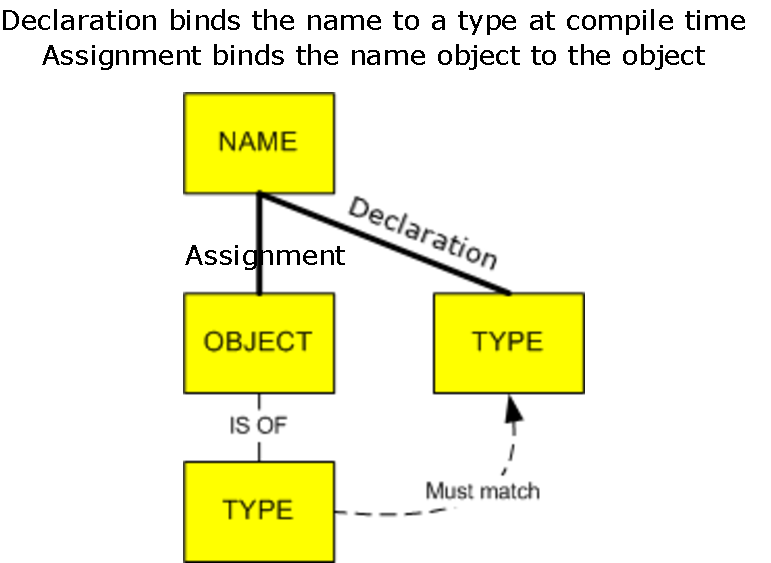
\includegraphics[scale=0.4]{figs/static_typing.pdf}
    %\hspace{1em}
    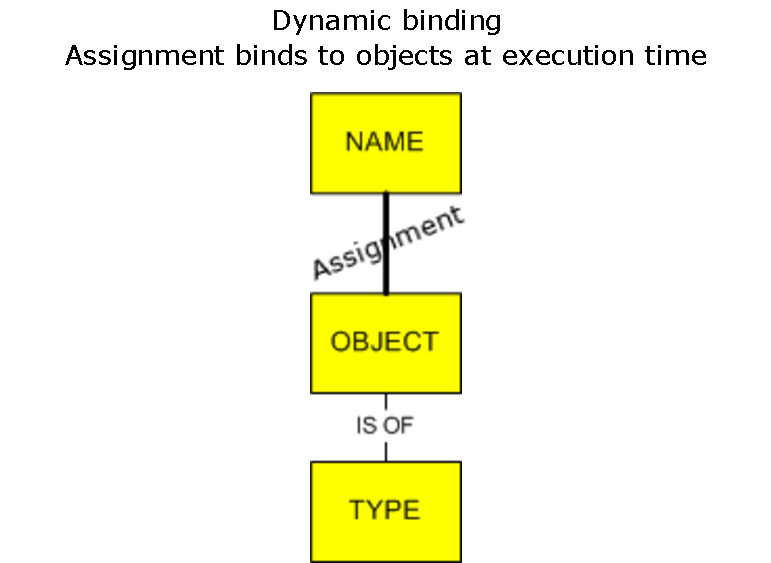
\includegraphics[scale=0.4]{figs/dynamic_typing.pdf}
    \end{center}

    Therefore, one variable name can be reused for different objects. Variable assignment is done with the \verb+=+ sign:
    \lstinputlisting[linerange={1-3}, basicstyle=\ttfamily\scriptsize]{scripts/vars.py}

\end{frame}


\begin{frame}[fragile]
    \frametitle{Variables as objects}

    Python is object oriented. Therefore, each assigned variable is an object, about which informations are accessible via:
    \lstinputlisting[linerange={4-6}, basicstyle=\ttfamily\scriptsize]{scripts/vars.py}

    There are of two main caterogies of objects: (source: \href{https://www.geeksforgeeks.org/mutable-vs-immutable-objects-in-python/}{geeksforgeeks}): \\
    \begin{itemize}
        \item{\emph{Mutable objects}: Can't change their state and contents: \textbf{list, dict, set}}
        \item{\emph{Immutable objects}: Can change their state and contents: \textbf{int, float, bool, string, unicode, tuple and custom objects}}
    \end{itemize}

%For instance, although strings are in practice close to a list, the following statement
%    \lstinputlisting[linerange={5-6}, basicstyle=\ttfamily\scriptsize]{scripts/vars.py} 
%    will return
%    \begin{lstlisting}[basicstyle=\ttfamily\scriptsize]
%Traceback (most recent call last):
%  File "vars.py", line 6, in <module>
%    x[0] = 1
%TypeError: 'str' object does not support item assignment
%    \end{lstlisting}
\end{frame}

%\begin{frame}[fragile]
%    \frametitle{Mutable and immutable objects}
%    This is important when looking at assignments for instance. The following:
%    \lstinputlisting[linerange={8-12}, basicstyle=\ttfamily\scriptsize]{scripts/vars.py} 
%    will return 
%    \begin{lstlisting}[basicstyle=\ttfamily\scriptsize]
%x =  [0, 1, 2] y =  [0, 1, 2]
%x =  [0, 'oups', 2] y =  [0, 'oups', 2]
%    \end{lstlisting}
%    The change in \verb+x+ is visible in \verb+y+. Indeed, copy assignments copy \emph{references} (i.e. memory adresses), which is not modified in that case.
%\end{frame}
